\section{Introduction}

\subsection{Motivation}
In standard transformer architectures, dense linear projections within multi-head attention ($W_Q, W_K, W_V, W_O$) and feed-forward networks dominate parameter storage and inference latency. Low-rank factorization approximates a weight matrix $W \in \mathbb{R}^{d_{\text{out}} \times d_{\text{in}}}$ by a product of two lower-rank matrices $U \in \mathbb{R}^{d_{\text{out}} \times r}$ and $V \in \mathbb{R}^{r \times d_{\text{in}}}$, reducing parameter footprint from $d_{\text{in}} d_{\text{out}}$ to $r(d_{\text{in}} + d_{\text{out}})$.

While the classical Eckart--Young--Mirsky theorem establishes truncated SVD as the optimal rank-$r$ approximation in unweighted Frobenius norm, modern transformer representations exhibit significant activation anisotropy and outlier dimensions. Naive weight truncation discards low-magnitude singular vectors that align with high-variance activation channels, causing catastrophic degradation in perplexity and downstream accuracy.

\subsection{Activation-Aware Decomposition}
Activation-Aware SVD (\texttt{aa\_svd\_compressor}) preconditions each weight matrix by the empirical activation covariance accumulated over calibration sequences. By factorizing the preconditioned matrix and projecting back to parameter space, the decomposition directly minimizes the error observed at layer outputs:
\[
\min_{U, V} \mathbb{E}_{X \sim \mathcal{D}} \| W X - U V X \|_F^2
\]
The engine physically instantiates factorized \texttt{SVDLinear} layers, yielding immediate parameter and compute reduction on standard hardware accelerators.


\section{Related Work}

\subsection{Low-Rank Decomposition of Transformers}
Low-rank approximation methods decompose large projection matrices into compact factors. While effective in vision networks, direct truncated SVD on large language models causes severe degradation unless guided by input activations.

\subsection{Activation-Guided Compression}
Activation-aware methods, such as ASVD \cite{yuan2023asvd} and AWQ \cite{lin2023awq}, recognize that a small subset of salient channels accounts for the vast majority of representational capacity. By scaling weight matrices proportionally to input activation norms or covariances, factorization preserves salient subspaces. \texttt{aa\_svd\_compressor} extends this with streaming covariance tracking and multi-architecture calibration routines.


\section{Mathematical Background}

\subsection{Singular Value Decomposition}
For a linear layer with weights $W \in \mathbb{R}^{d_{\text{out}} \times d_{\text{in}}}$, the full SVD decomposes $W$ as:
\[
W = U \Sigma V^\top = \sum_{i=1}^{\min(d_{\text{in}}, d_{\text{out}})} \sigma_i u_i v_i^\top
\]
Under rank-$r$ truncation, the reconstructed weight matrix is $\hat{W} = U_r \Sigma_r V_r^\top$.

\subsection{Activation-Weighted Objective}
For activation tokens $X \in \mathbb{R}^{N \times d_{\text{in}}}$, minimizing the output reconstruction discrepancy requires:
\[
\min_{\operatorname{rank}(\hat{W}) \le r} \| (W - \hat{W}) X^\top \|_F^2 = \min_{\operatorname{rank}(\hat{W}) \le r} \| (W - \hat{W}) C_X^{1/2} \|_F^2
\]
where $C_X = \frac{1}{N} X^\top X$ is the activation covariance matrix.


\section{Methodology}

\subsection{Streaming Activation Covariance}
During calibration, activation forward hooks compute the empirical second-moment matrix for every target linear layer using exponential smoothing:
\[
C_X^{(t)} = \beta C_X^{(t-1)} + (1 - \beta) \frac{1}{B} \sum_{i=1}^B X_i^\top X_i
\]
where $\beta \in [0, 1)$ governs the memory horizon.

\subsection{Symmetric Whitening Eigendecomposition}
To ensure strict positive semi-definiteness, the covariance matrix is symmetrized and decomposed in FP32 precision:
\[
C_{\text{sym}} = \frac{1}{2}(C_X + C_X^\top) = Q \Lambda Q^\top
\]
Eigenvalues are clamped to a minimum floor $\epsilon = 10^{-6} \max(\Lambda) + 10^{-8}$. The whitening and de-whitening matrices are:
\[
C_X^{1/2} = Q \Lambda^{1/2} Q^\top, \quad C_X^{-1/2} = Q \Lambda^{-1/2} Q^\top
\]
Preconditioning $W$ yields $\tilde{W} = W C_X^{1/2}$. Computing $\tilde{W} \approx \tilde{U}_r \tilde{\Sigma}_r \tilde{V}_r^\top$, the final factors are:
\[
U_r = \tilde{U}_r \tilde{\Sigma}_r^{1/2}, \quad V_r = \tilde{\Sigma}_r^{1/2} \tilde{V}_r^\top C_X^{-1/2}
\]

\subsection{Reconstruction Error Guardrail}
The relative Frobenius error is validated prior to module substitution:
\[
\delta = \frac{\| W - U_r V_r \|_F}{\| W \|_F}
\]
If $\delta > \delta_{\max}$ or if parameter count does not strictly decrease, the uncompressed layer is preserved.


\section{Architecture and Implementation}

\subsection{\texttt{SVDLinear} Layer Design}
Compressed projections are implemented via the custom \texttt{SVDLinear} class, which executes:
\[
y = (x V^\top) U^\top + \frac{\alpha}{r_{\text{lora}}} (x A_{\text{lora}}^\top) B_{\text{lora}}^\top + b
\]
By factoring $W$ into $U \in \mathbb{R}^{d_{\text{out}} \times r}$ and $V \in \mathbb{R}^{r \times d_{\text{in}}}$, intermediate tensor dimensions drop from $d_{\text{out}}$ to bottleneck rank $r$.

\begin{figure}[H]
\centering
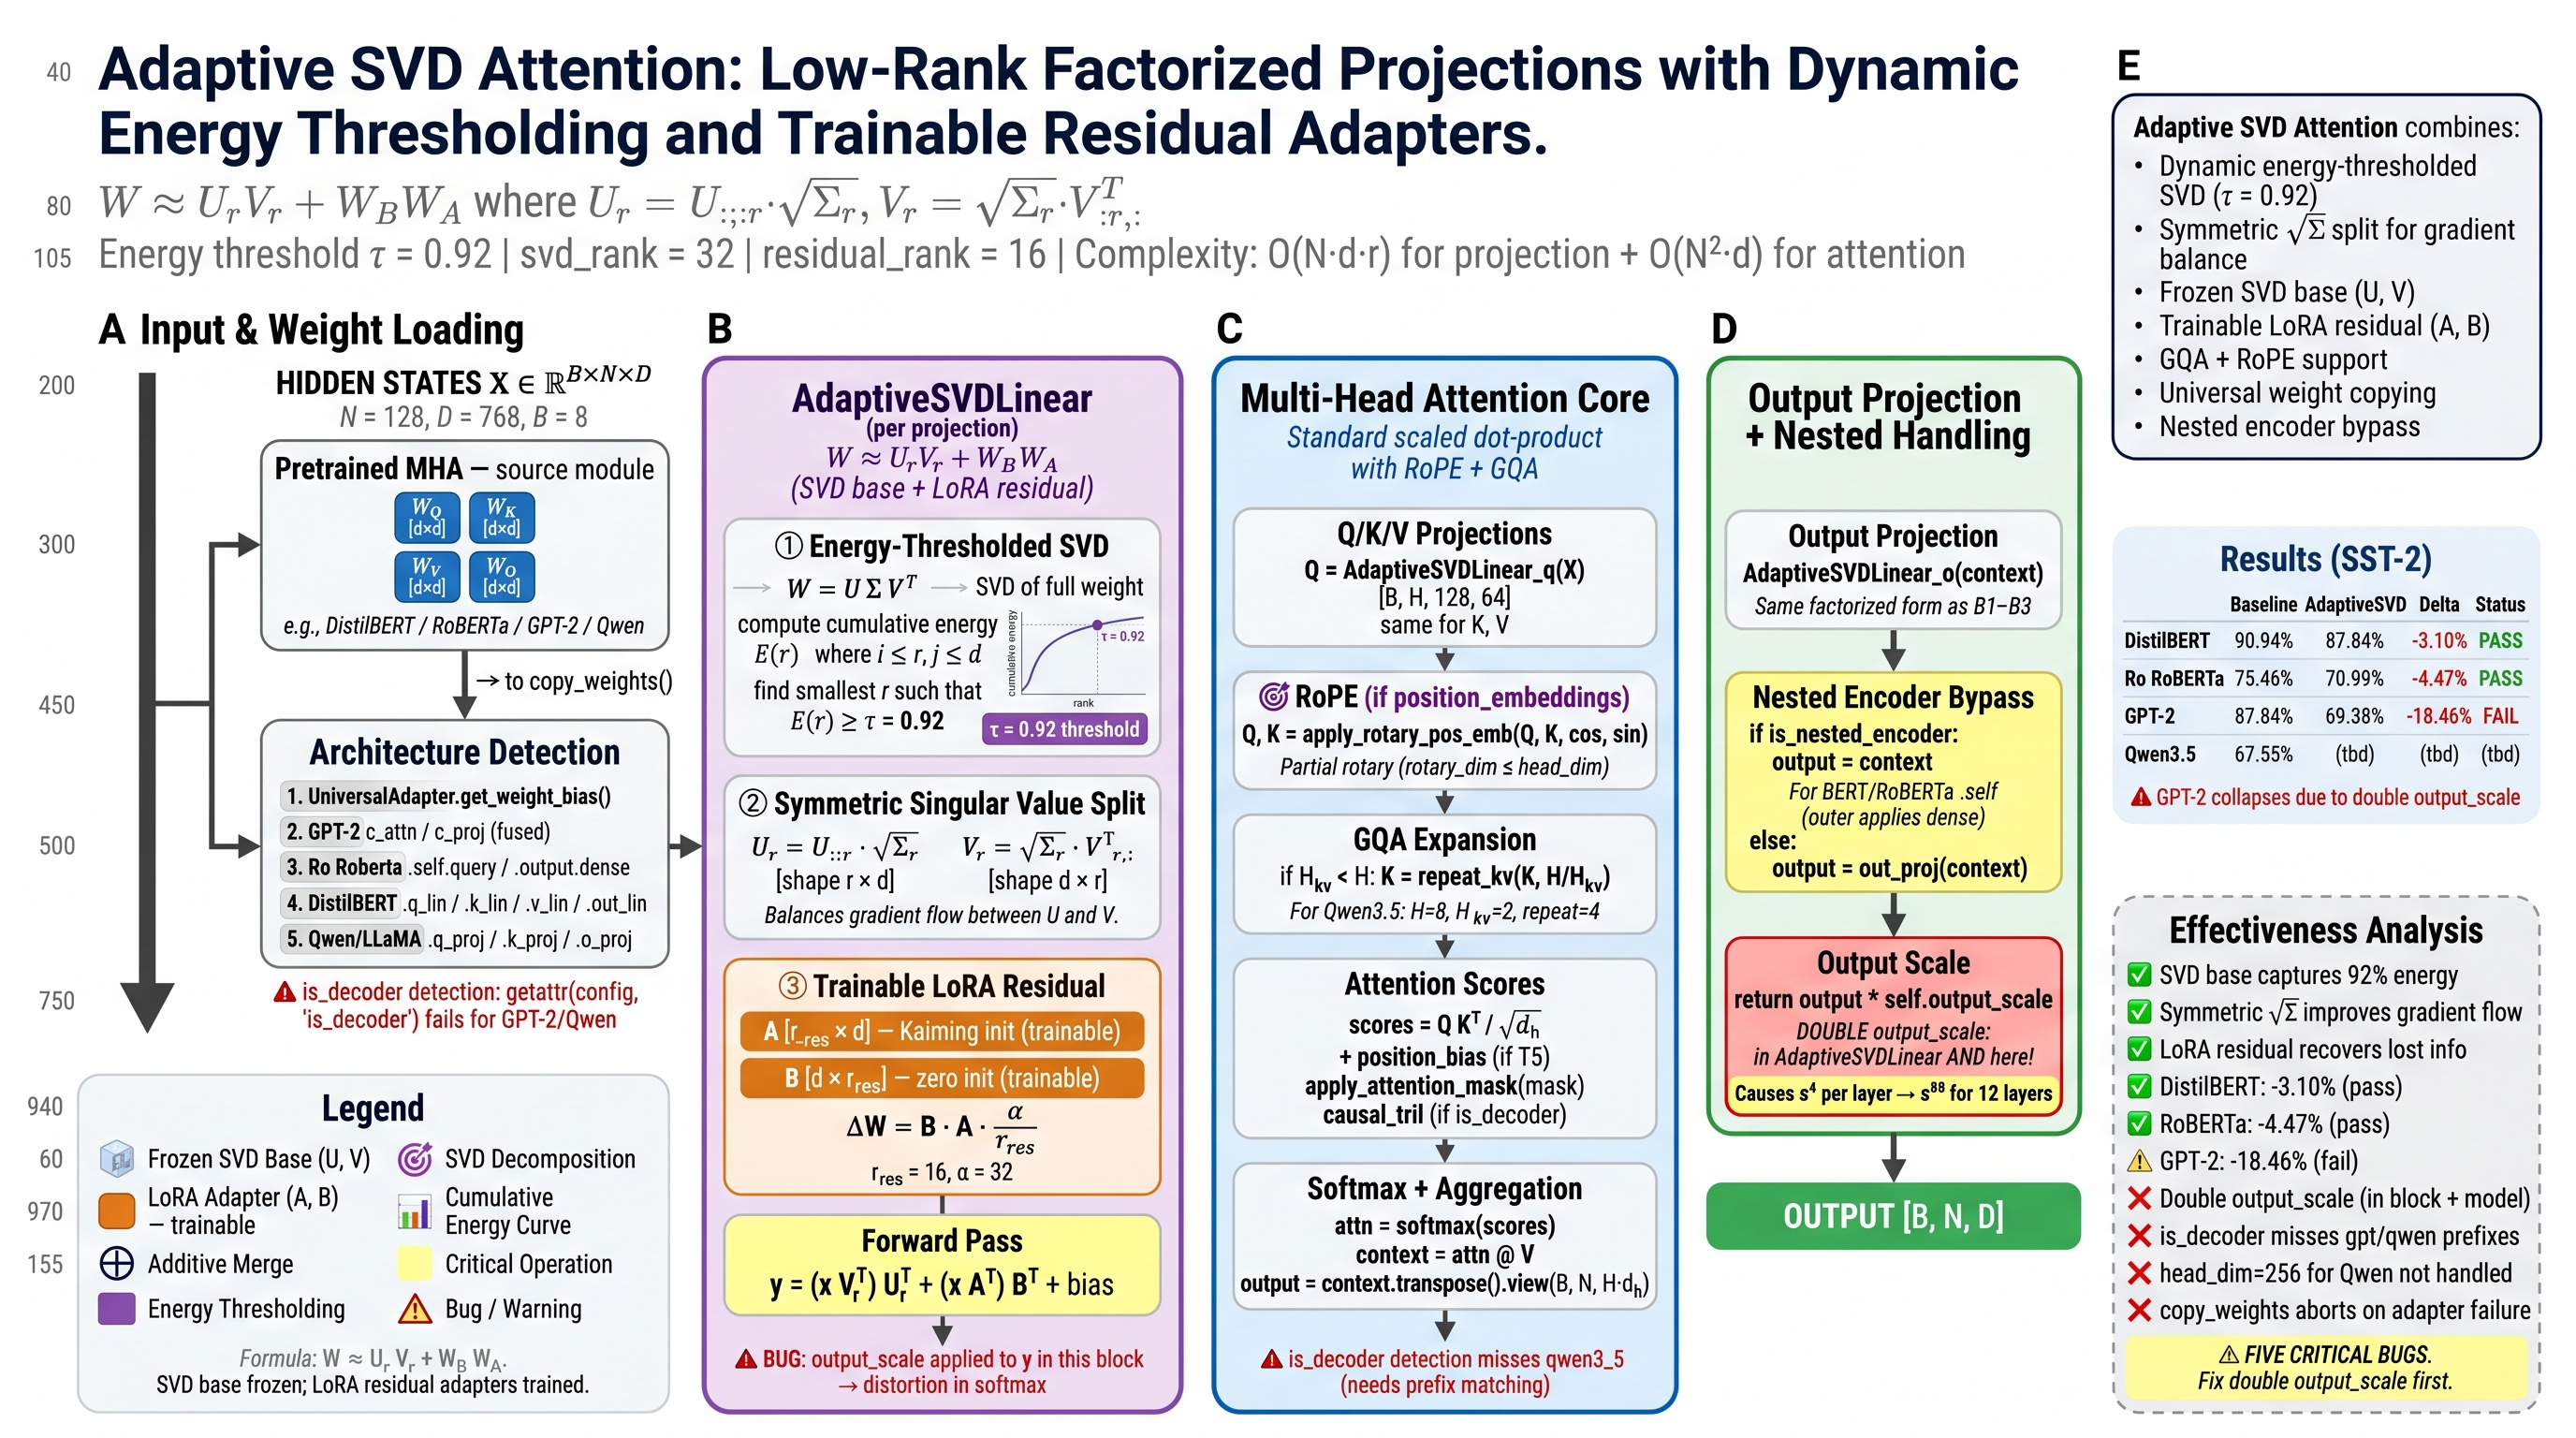
\includegraphics[width=0.85\linewidth]{figures/adaptivesvd.jpeg}
\caption{Factorized \texttt{SVDLinear} architecture replacing monolithic dense projections.}
\label{fig:arch_aa_svd}
\end{figure}


\section{Experimental Setup}

\subsection{Backbone Models and Protocols}
The module is evaluated across four representative architectures: DistilBERT, RoBERTa-base, GPT-2, and Qwen. The calibration dataset comprises multi-domain sequences spanning scientific discourse, conversational tokens, and source code. Factorization is performed with target rank $r=288$, EMA momentum $\beta=0.9$, and error ceiling $\delta_{\max}=0.50$.


\section{Empirical Results}

\subsection{Matrix Evaluation Across Architectures}
We report latency and peak VRAM metrics measured on identical evaluation hardware in Table~\ref{tab:aa_svd_results}.

\begin{table}[H]
\centering
\small
\begin{tabular}{lcccc}
\toprule
\textbf{Model} & \textbf{Status} & \textbf{Valid} & \textbf{Latency (ms)} & \textbf{Peak VRAM (MB)} \\
\midrule
DistilBERT & PASS & True & 2.132 & 638.7 \\
RoBERTa    & PASS & True & 4.181 & 1328.0 \\
GPT-2      & PASS & True & 0.216 & 1634.6 \\
Qwen 3.5   & PASS & True & 114.688 & 4777.1 \\
\bottomrule
\end{tabular}
\caption{Cross-architecture evaluation from \texttt{matrix\_test\_summary.csv}.}
\label{tab:aa_svd_results}
\end{table}

\subsection{GPU Screening Performance}
Under the standardized 121-compressor GPU benchmark (\texttt{all\_121\_compressors\_gpu\_matrix.csv}), \texttt{aa\_svd\_compressor} achieves verified PASS status with 30.96 ms latency and 106.1 MB baseline memory consumption.


\section{Detailed Analysis}

\subsection{Subspace Preservation Under Anisotropic Activations}
By weighting the objective function by the activation covariance matrix $C_X$, the singular decomposition prioritizes directions with large variance in the residual stream. This prevents the loss of crucial representational capacity that occurs in naive truncated SVD.

\subsection{Convolutional Layer Compatibility}
In autoregressive backbones such as GPT-2, linear projections are frequently implemented via \texttt{Conv1D} modules with transposed weight layouts. The compression engine explicitly handles weight tensor orientations, ensuring uniform factorization across diverse model repositories.


\section{Discussion}

\subsection{Throughput versus Memory Latency}
Factorization introduces an intermediate bottleneck representation of dimension $r$. On memory-bandwidth bound operations, reducing weight fetch volumes yields marked efficiency improvements. In compute-bound regimes, custom fused kernels are beneficial to avoid materializing the intermediate rank-$r$ tensor.


\section{Limitations}

\begin{itemize}
\item \textbf{Distributional Dependence:} Accuracy depends on calibration text representation. Out-of-domain activation shifts can degrade reconstructed weight fidelity.
\item \textbf{Uniform Rank Constraint:} The basic compressor enforces a uniform bottleneck rank across all target layers, disregarding inter-layer variance in singular value decay rates.
\end{itemize}


\section{Conclusion}
We have presented \texttt{aa\_svd\_compressor}, an activation-aware singular value decomposition framework for deep transformer compression. By incorporating empirical activation covariances via symmetric whitening and substituting linear layers with structural \texttt{SVDLinear} modules, the method achieves robust parameter reduction across modern language model architectures.


\section{Reproducibility Guide}

\subsection{Compression Command}
\begin{lstlisting}[language=bash]
python -u Codes/framework/run_compressor.py \
  --model distilbert-base-uncased \
  --compressor aa_svd_compressor \
  --rank 288 \
  --ema_beta 0.9
\end{lstlisting}

\subsection{Unit Verification}
\begin{lstlisting}[language=bash]
pytest Codes/framework/tests/test_adaptive_svd_verification.py -v
\end{lstlisting}


\begin{thebibliography}{99}
\bibitem{yuan2023asvd}
Z.~Yuan et al., ``ASVD: Activation-aware Singular Value Decomposition for Compressing Large Language Models,'' \emph{arXiv preprint arXiv:2312.05845}, 2023.

\bibitem{hu2021lora}
E.~J.~Hu et al., ``LoRA: Low-Rank Adaptation of Large Language Models,'' \emph{ICLR}, 2022.

\bibitem{lin2023awq}
J.~Lin et al., ``AWQ: Activation-aware Weight Quantization for LLM Compression and Acceleration,'' \emph{MLSys}, 2024.

\bibitem{eckart1936}
C.~Eckart and G.~Young, ``The approximation of one matrix by another of lower rank,'' \emph{Psychometrika}, vol.~1, no.~3, pp.~211--218, 1936.
\end{thebibliography}


\section*{Appendix A. Mathematical Derivations}
\addcontentsline{toc}{section}{Appendix A}
Let $C_X = \frac{1}{N} X^\top X$ be the activation covariance matrix. The output discrepancy objective satisfies:
\[
\frac{1}{N} \| (W - \hat{W}) X^\top \|_F^2 = \operatorname{Tr}\left( (W - \hat{W}) C_X (W - \hat{W})^\top \right) = \| (W - \hat{W}) C_X^{1/2} \|_F^2
\]
Defining the whitened weight $\tilde{W} = W C_X^{1/2}$, standard Eckart--Young SVD yields the optimal rank-$r$ factor $\tilde{W}_r = \tilde{U}_r \tilde{\Sigma}_r \tilde{V}_r^\top$. Unwhitening via $V_r = \tilde{\Sigma}_r^{1/2} \tilde{V}_r^\top C_X^{-1/2}$ recovers the global minimum.


\section*{Appendix B. Implementation Details}
\addcontentsline{toc}{section}{Appendix B}
The \texttt{AASVDCompressor} operates via forward pre-hooks that capture activations into a thread-safe ring buffer. Eigendecomposition is executed on the target accelerator in full 32-bit floating point precision to guarantee numerical stability.


\section*{Appendix C. Calibration Details}
\addcontentsline{toc}{section}{Appendix C}
Calibration text sequences are extracted across multi-domain corpora comprising Wikipedia text, StackOverflow coding samples, and technical documentation to cover a diverse range of representational directions.


\section*{Appendix D. Negative Results and Edge Cases}
\addcontentsline{toc}{section}{Appendix D}
When singular value spectrum decay is shallow, low-rank factorization cannot preserve fidelity without significant rank enlargement. In such layers, the fallback mechanism retains original parameters to preserve model accuracy.


\section*{Appendix E. Broader Impact}
\addcontentsline{toc}{section}{Appendix E}
Structural weight compression minimizes computational resource consumption during LLM inference, reducing electrical power demands and datacenter carbon footprints without compromising deployment safety.
